\section{Recurrent Networks}

Map time into state.

Elman's network:
\begin{itemize}
  \item Next word prediction (29 word bank)
  \item backprop only one step back in time
\end{itemize}

RNNs have the vanishing/exploding gradient problem. In backprop, grad is multiplied by weights
at each layer, so if the weights are < 1, the gradient may vanish and long term dependencies can't
be learned. Otherwise, it may explode, and wont converge.

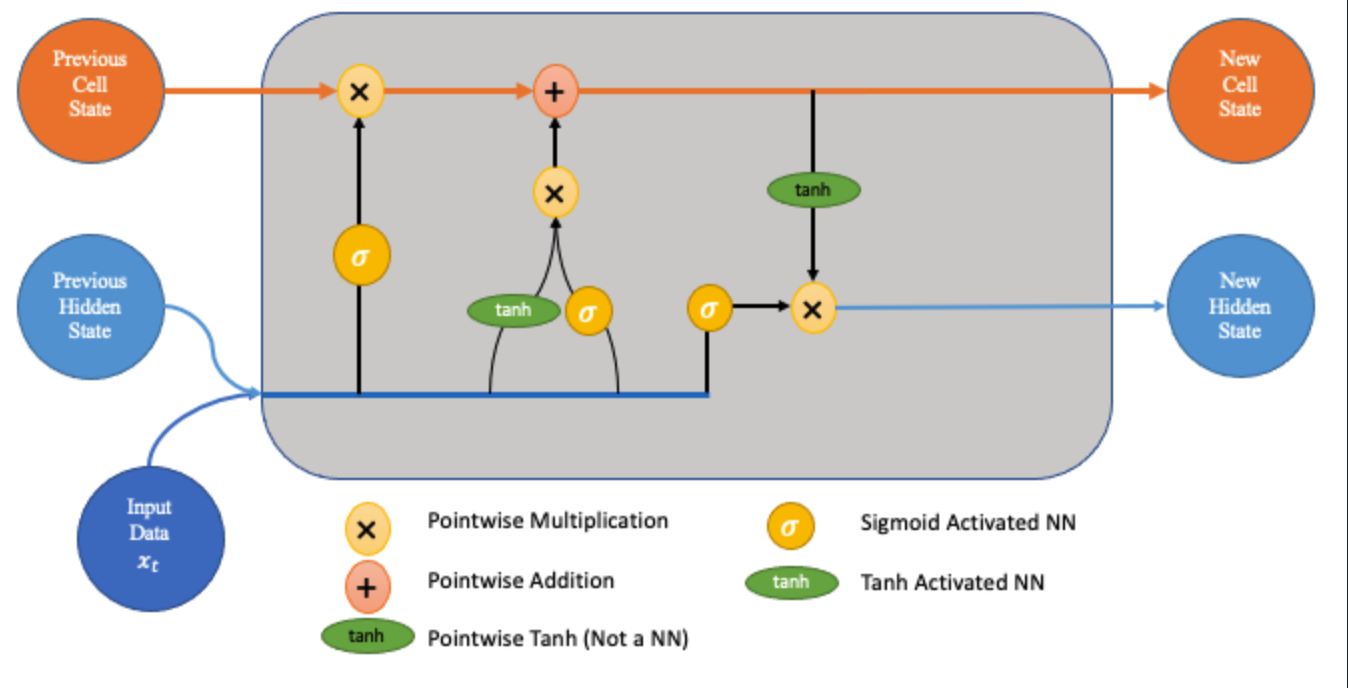
\includegraphics[width=0.9\columnwidth]{images/lstm}

Forget, input, and output gates (left to right).

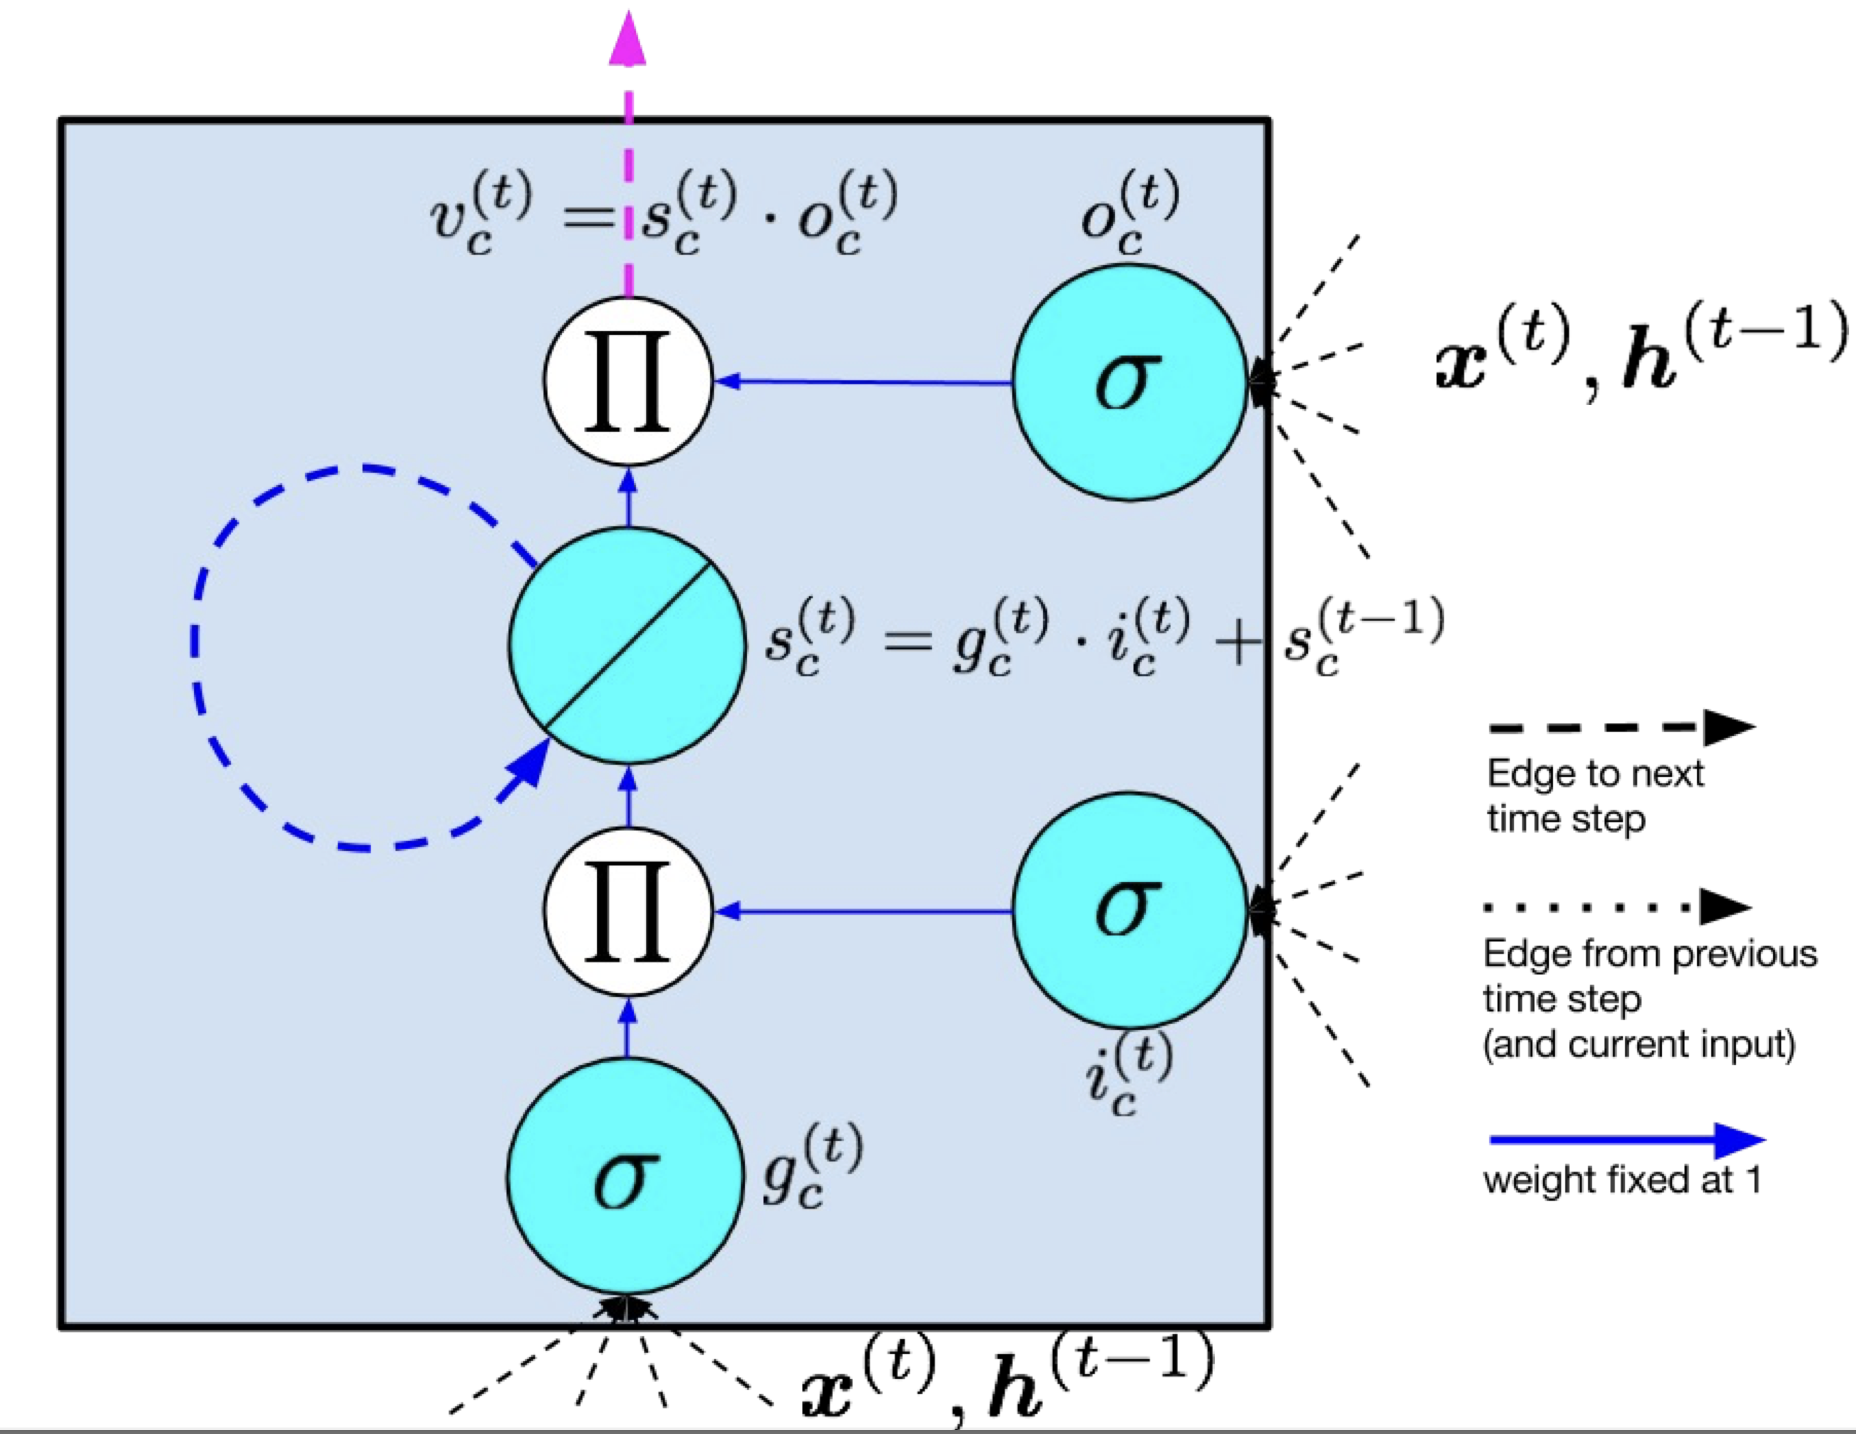
\includegraphics[width=0.9\columnwidth]{images/memcell}
